\documentclass{article}

\usepackage[margin=.75in]{geometry}
\usepackage{amsmath}
\usepackage{amssymb}
\usepackage[shortlabels]{enumitem}
\usepackage{float}
\usepackage{verbatim}
\usepackage{caption}
\usepackage{subcaption}
\usepackage{tikz}
\usetikzlibrary{shapes,arrows,positioning,calc}

\usepackage{mathtools}
\DeclarePairedDelimiter\norm{\lVert}{\rVert}%

\author{Anthony Siddique, Damien Prieur, Jachin Philip, Obinna Ekeh}
\title{Homework 6\\ MEM 633 \\ Group 1}
\date{}

\begin{document}

\maketitle

\section*{Problem 1}
Run the program several times with random initial conditions to verify that
$x = \bar{x}_U = \begin{bmatrix} 0 & 0 & x_3 & 0 \end{bmatrix}^T, u = \bar{y} = 0$
and $x = \bar{x}_s = \begin{bmatrix} \pi & 0 & x_3 & 0 \end{bmatrix}^T, u = \bar{u} = 0$,
where $x_3$ can be any constant.
\newline
\newline
After running a few random starting conditions we can see that
$ x = \begin{bmatrix} 0 & 0 & x_3 & 0 \end{bmatrix} $
is a stable equilibrium as all starting points go to this state except the one starting at the other equilibrium.
This matches what we expect, the pendulum in the downward position is the stable equilibrium of the uncontrolled system.
The other equilibrium point is the pendulum being perfectally vertical, but that is unstable as any small perterbation will cause the uncontrolled system to go to the other equilibirum state.
\begin{figure}[htb]
\centering
\begin{subfigure}{0.49\linewidth} \centering
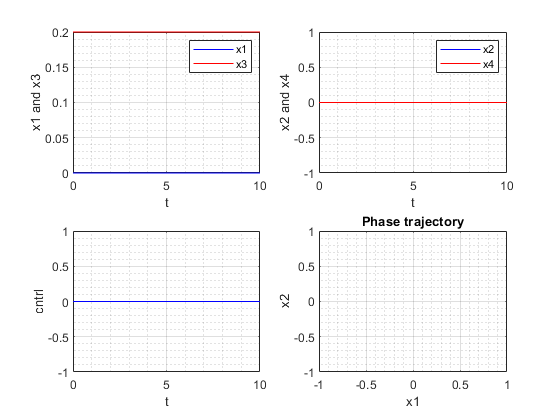
\includegraphics[scale=.6]{images/p1-vertical.png}
\caption*{$x(0) = \begin{bmatrix} 0 & 0 & 0 & 0 \end{bmatrix}^T$}
\end{subfigure}
\begin{subfigure}{0.49\linewidth} \centering
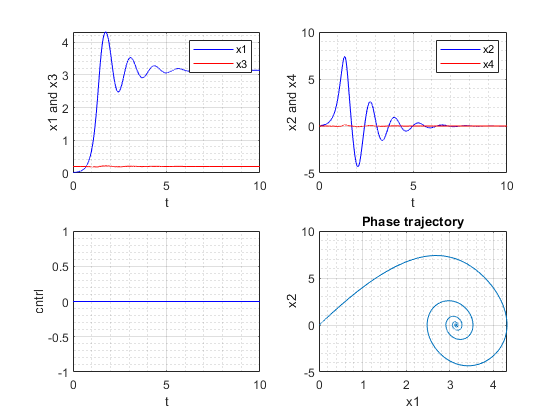
\includegraphics[scale=.6]{images/p1-slightly-off.png}
\subcaption*{$x(0) = \begin{bmatrix} 1 & 0 & 0 & 0 \end{bmatrix}^T$}
\end{subfigure}
\end{figure}


\section*{Problem 2}
Let the initial conditions be $x_{10} = 0.26rad$, $x_{30} = .2m$, and run the program with at least the following seven state feedback controllers.
\newline
\begin{minipage}{0.45\textwidth}
$$ F_1 = \begin{bmatrix} 120 & 22 & 20 & 28 \end{bmatrix} $$
$$ F_2 = \frac{1}{2}\begin{bmatrix} 120 & 22 & 20 & 28 \end{bmatrix} $$
$$ F_3 = \begin{bmatrix} 120 & 22 & 0 & 28 \end{bmatrix} $$
$$ F_4 = \begin{bmatrix} 90 & 22 & 20 & 28 \end{bmatrix} $$
\end{minipage}
\begin{minipage}{0.45\textwidth}
$$ F_5 = \begin{bmatrix} 60 & 22 & 20 & 28 \end{bmatrix} $$
$$ F_6 = \begin{bmatrix} 0 & 22 & 20 & 28 \end{bmatrix} $$
$$ F_7 = \begin{bmatrix} 0 & 0 & 0 & 0 \end{bmatrix} $$
\end{minipage}
\newline
\newline
\begin{enumerate}[1)]
\item $$ F_1 = \begin{bmatrix} 120 & 22 & 20 & 28 \end{bmatrix} $$
\begin{minipage}{\linewidth}
\centering
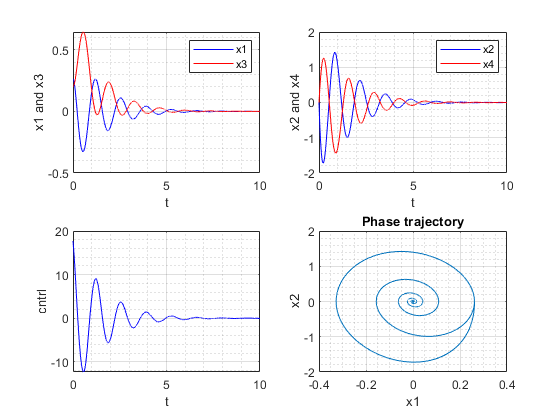
\includegraphics[scale=.8]{images/p2-1.png}
\end{minipage}
We can see that the system is controlled and reaches it's equilibirum by 5 seconds and most of the action occurs in the first 2 seconds.
The largest input is about 35 units.
Using this as our base point for the other models we can make qualitative claims about the data.

\item $$ F_2 = \frac{1}{2}\begin{bmatrix} 120 & 22 & 20 & 28 \end{bmatrix} $$
\begin{minipage}{\linewidth}
\centering
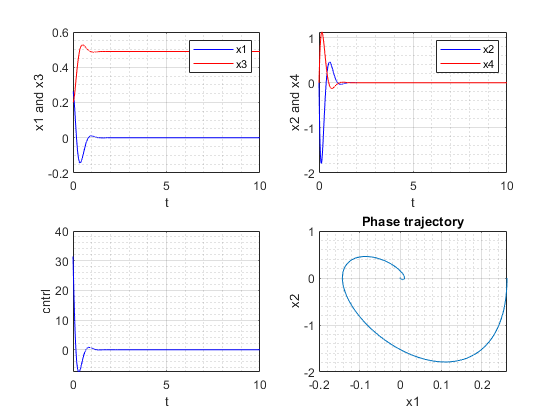
\includegraphics[scale=.8]{images/p2-2.png}
\end{minipage}
This system while stable and reaches it's equilibirum has a lot of oscillations.
It consistantly overshoots the equilibirum point, and the control is visibly oscillating through the end of the simulation.
By contrast the max input was about 17 so there is a tradeoff.
The system is just reacting too slowly the the current state of the system which makes sense as it's just half of the first.

\newpage
\item $$ F_3 = \begin{bmatrix} 120 & 22 & 0 & 28 \end{bmatrix} $$
\begin{minipage}{\linewidth}
\centering
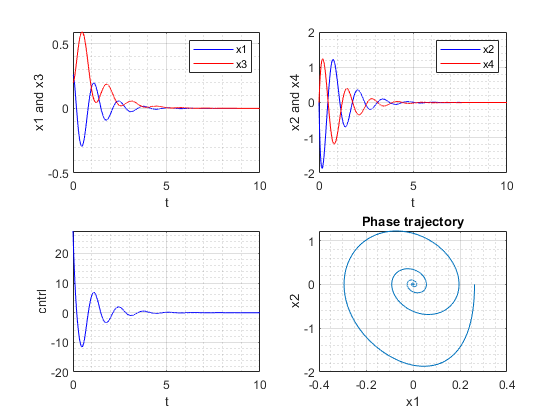
\includegraphics[scale=.8]{images/p2-3.png}
\end{minipage}
This system is stable other than the position of the cart.
It appears to behave very similarly to the first system other than the location of the cart not being brought to zero.
This is expected as it's gain is set to zero.

\item$$ F_4 = \begin{bmatrix} 90 & 22 & 20 & 28 \end{bmatrix} $$
\begin{minipage}{\linewidth}
\centering
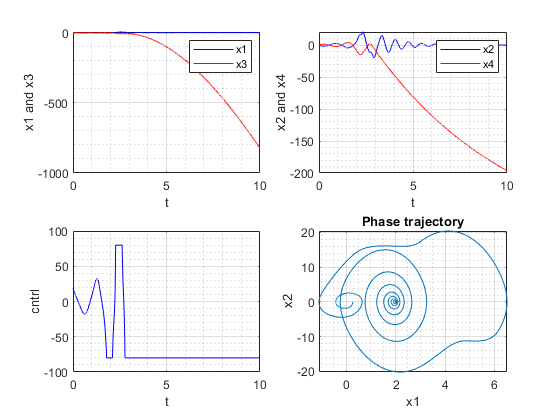
\includegraphics[scale=.8]{images/p2-4.png}
\end{minipage}
This system oscillates like the second system, but it reaches a steady steate a bit sooner.
It is still reacting too slowly to the most sensitive variable in our system, the angle of the pendulum.

\newpage
\item $$ F_5 = \begin{bmatrix} 60 & 22 & 20 & 28 \end{bmatrix} $$
\begin{minipage}{\linewidth}
\centering
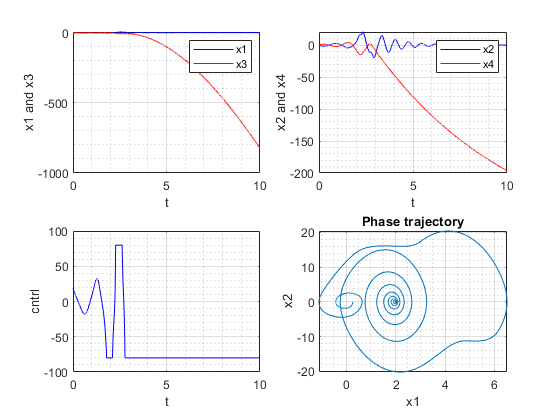
\includegraphics[scale=.8]{images/p2-5.png}
\end{minipage}
This system is clearly unstable, it tries but is unable to keep the pendulum vertical.
It doesn't react to the pendulum angle fast enough and quickly leaves the linearized reagion.

\item $$ F_6 = \begin{bmatrix} 0 & 22 & 20 & 28 \end{bmatrix} $$
\begin{minipage}{\linewidth}
\centering
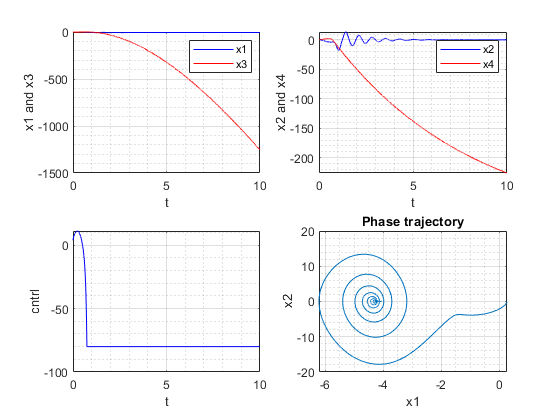
\includegraphics[scale=.8]{images/p2-6.png}
\end{minipage}
This system is also unstable, but it should just ignore the angle of the pendulum and return the cart to the origin.
Due to the linearlization region leading to flipped signs once the pendulum has fallen the cart tries to stop the angular velocity of the pendulum but it is doing so incorrectly.
This leads to the cart just driving away.

\newpage
\item $$ F_7 = \begin{bmatrix} 0 & 0 & 0 & 0 \end{bmatrix} $$
\begin{minipage}{\linewidth}
\centering
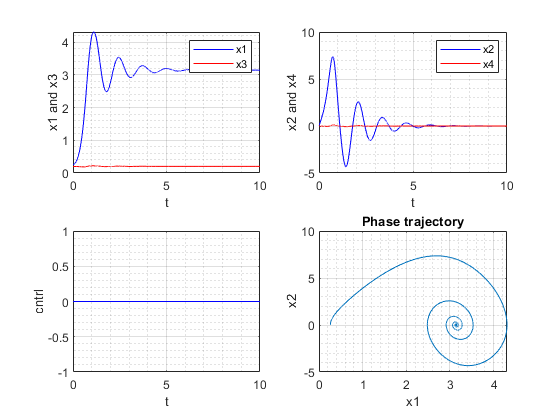
\includegraphics[scale=.8]{images/p2-7.png}
\end{minipage}
This system is the system with no input and we know this system is unable to keep the pendulum vertical and makes no effort at correcting the cart's position.
\end{enumerate}

\section*{Problem 3}
The linearized state equation at the equilibrium $ x = \hat{x}_u = \begin{bmatrix} 0 & 0 & 0 & 0 \end{bmatrix}^T$ is given by
$$ \dot{x}(t) = Ax(t) + Bu(t) $$
where
$$
A_0 =
\begin{bmatrix}
0 & 1 & 0 & 0 \\
25.15 & 0 & 0 & 0 \\
0 & 0 & 0 & 1 \\
-0.42094 & 0 & 0 & 0 \\
\end{bmatrix}
, \quad
B =
\begin{bmatrix}
0 \\
-1.3547 \\
0 \\
0.5504 \\
\end{bmatrix}
$$
If the frictions are negligible and
$$
A_f =
\begin{bmatrix}
0 & 1 & 0 & 0 \\
25.15 & -1.6188 & 0 & 0.33868 \\
0 & 0 & 0 & 1 \\
-0.42094 & 0.027094 & 0 & -0.1376 \\
\end{bmatrix}
, \quad
B =
\begin{bmatrix}
0 \\
-1.3547 \\
0 \\
0.5504 \\
\end{bmatrix}
$$
If the frictions are considered.
\newline
Compute the eigenvalues of $A_0 + BF$ and $A_f + BF$ for each of the seven cases in the previous problem and explain their physical meanings and relevance to the simulation results.
\newline
\newline
\begin{enumerate}[1)]
\item
$$ eig(A_0 + BF) =
\begin{bmatrix}
-5.0895 + 7.3694i \\
-5.0895 - 7.3694i \\
-1.0444 \\
-3.1688 \\
\end{bmatrix}
\qquad
eig(A_f + BF) =
\begin{bmatrix}
-8.4917 \\
-3.3238 + 4.4634i \\
-3.3238 - 4.4634i \\
-1.0094 \\
\end{bmatrix}
$$
We can see that all the poles are in the left-half plane so our system is stable.
\item
$$ eig(A_0 + BF) =
\begin{bmatrix}
-1.1202 + 5.8792i \\
-1.1202 - 5.8792i \\
-0.9176 \\
-4.0381 \\
\end{bmatrix}
\qquad
eig(A_f + BF) =
\begin{bmatrix}
-0.7221 + 4.6353i \\
-0.7221 - 4.6353i \\
-6.5937 \\
-0.9146 \\
\end{bmatrix}
$$
We can see that the system is once again stable, but the real value of the poles are much smaller, closer to zero.
Due to this the response is going to be slower, and the oscillatory components will be able to be seen much more.
\item
$$ eig(A_0 + BF) =
\begin{bmatrix}
0 \\
-5.2792 + 8.3106i \\
-5.2792 - 8.3106i \\
-3.8337 \\
\end{bmatrix}
\qquad
eig(A_f + BF) =
\begin{bmatrix}
0 \\
-7.5489 \\
-4.2998 + 5.5046i \\
-4.2998 - 5.5046i \\
\end{bmatrix}
$$
One variable is not stable. If we were to look at the eigenvector associated with this eigenvalue we would see it's with the position vector.
Since the gain is zero for it we are ignoring its value, but the system will otherwise behave very similarly to the first as it has very similar eigenvalues otherwise.
\item
$$ eig(A_0 + BF) =
\begin{bmatrix}
-9.1035 \\
-2.2130 + 5.3762i \\
-2.2130 - 5.3762i \\
-0.8627 \\
\end{bmatrix}
\qquad
eig(A_f + BF) =
\begin{bmatrix}
-13.3599 \\
-0.9651 + 4.7131i \\
-0.9651 - 4.7131i \\
-0.8585 \\
\end{bmatrix}
$$
This system is stable, but has very small real components for the eigenvalues of the friction system which is a better approximation of the actual simulation.
Due to this the system will react slowly and be dominated by the oscillatory motions before eventually dampening out.
\item
$$ eig(A_0 + BF) =
\begin{bmatrix}
-12.9993 \\
-0.3117 + 5.1420i \\
-0.3117 - 5.1420i \\
-0.7695 \\
\end{bmatrix}
\qquad
eig(A_f + BF) =
\begin{bmatrix}
-16.1090 \\
0.3662 + 4.6056i \\
0.3662 - 4.6056i \\
-0.7720 \\
\end{bmatrix}
$$
The non friction model would lead us to believe the system is stable, but we can see that even with a linearlized model of the friction case we are unstable.
\item
$$ eig(A_0 + BF) =
\begin{bmatrix}
-17.5981 \\
1.9335 + 4.3679i \\
1.9335 - 4.3679i \\
-0.6611 \\
\end{bmatrix}
\qquad
eig(A_f + BF) =
\begin{bmatrix}
-19.9892 \\
2.2538 + 3.8513i \\
2.2538 - 3.8513i \\
-0.6669 \\
\end{bmatrix}
$$
This system is just unstable, but we would expect the system to have some stabiled eigenvectors, but since the system is nonlinear we will leave the region where the linearization can be useful.
This may leave the system with no stable coordinates.
\item
$$ eig(A_0 + BF) =
\begin{bmatrix}
0 \\
0 \\
5.0150 \\
-5.0150 \\
\end{bmatrix}
\qquad
eig(A_f + BF) =
\begin{bmatrix}
0 \\
-5.8926 \\
4.2682 \\
-0.1319 \\
\end{bmatrix}
$$
This system is unstable, as we expect.
We are applying no input to the system so we expect the system to remain near its starting location with the cart oscillating a bit as the pendulum falls.
\end{enumerate}

\end{document}
